% In this talk, I’ll talk about how we can use silly games to understand the strengths and weaknesses of AIs. We first begin with games that test memory: testing the recall of obscure facts. While AI has been viewed as superhuman at this task, it isn’t universally so. We show that a new measure of adversarial datasets (the gap between humans and computers) is decreasing but not yet closed, with computers still struggling on abstract reasoning and knowing when they know the correct answer. Given these disparate skill sets, we then analyze how we can best build human and computer teams ito learn new facts and detect false statements. Finally, I close with a similar line of results for another silly language game, Diplomacy, where computers have still not reached dominance but can be used to assist human players think strategically and detect lies.”

\documentclass[compress]{beamer}

%\usepackage{beamerthemesplit}
\usepackage{xmpmulti}

\usepackage{booktabs}
\usepackage{xfrac}
\usepackage{graphicx,float,wrapfig, bbm}
\usepackage{amsfonts, bbold, comment}
\usepackage{mdwlist}
\usepackage{subfigure}
\usepackage{colortbl}
\usepackage{overpic}
\usepackage{pdfpages}
\usepackage[normalem]{ulem}
\usepackage{multirow}

\pgfdeclareimage[width=\paperwidth]{mybackground}{../../common/boulder.pdf}

\newcommand{\advscore}{\abr{AdvScore}}
\newcommand{\tif}[0]{\abr{tif}}
\newcommand{\twoplprob}[3]{ \frac{1}{1+\ex{-#3\left[ #1 - #2 \right] }  }}
\newcommand{\iif}{\abr{iif}}
\newcommand{\slda}[0]{\abr{slda}}
\newcommand{\bm}[1]{\mbox{\boldmath$#1$}}
\newcommand{\lda}[0]{\abr{lda}}
\newcommand{\explain}[2]{\underbrace{#2}_{\mbox{\footnotesize{#1}}}}
\newcommand{\itmspace}[0]{\hspace{2cm}}
\newcommand{\pos}[1]{{\texttt{#1}}}
\newcommand{\e}[2]{\mathbb{E}_{#1}\left[ #2 \right] }
\newcommand{\ind}[1]{\mathbb{I}\left[ #1 \right] }
\newcommand{\abr}[1]{\textsc{#1} }
\newcommand{\ex}[1]{\mbox{exp}\left\{ #1\right\} }
\newcommand{\g}{\, | \,}
\newcommand{\citename}[1]{#1 }
\newcommand{\fsi}[2]{
\begin{frame}[plain]
\vspace*{-1pt}
\makebox[\linewidth]{\includegraphics[width=\paperwidth]{#1}}
\begin{center}
#2
\end{center}
\end{frame}
}


\newcommand{\danquote}[1]{

\begin{flushright}
\begin{overpic}[width=5.5cm,tics=10]{general_figures/speech_bubble}
	\put(10,30) { \parbox{4cm}{#1 }}
\end{overpic}

\includegraphics[width=1.5cm]{general_figures/milkman_dan}
\end{flushright}
}


\newcommand{\gfxd}[2]{
	\begin{center}
		\includegraphics[width=#2\linewidth]{diplomacy/#1}
	\end{center}
}

\newcommand{\gfxt}[2]{
\begin{center}
	\includegraphics[width=#2\linewidth]{reading_tea_leaves/#1}
\end{center}
}

\newcommand{\gfxi}[2]{
\begin{center}
	\includegraphics[width=#2\linewidth]{interpretability/#1}
\end{center}
}

\newcommand{\gfxs}[2]{
\begin{center}
	\includegraphics[width=#2\linewidth]{simtrans/#1}
\end{center}
}

\newcommand{\gfxq}[2]{
\begin{center}
	\includegraphics[width=#2\linewidth]{qb/#1}
\end{center}
}


\newcommand{\gfxa}[2]{
	\begin{center}
		\includegraphics[width=#2\linewidth]{advcal/#1}
	\end{center}
}


\newcommand{\gfxu}[2]{
	\begin{center}
		\includegraphics[width=#2\linewidth]{uncertainty/#1}
	\end{center}
}

\newif\ifjobtalk\jobtalktrue
\newif\iflong\longtrue

\usetheme[
          showdate=true,                     % show the date on the title page
          alternativetitlepage=true,         % Use the fancy title page.
          titlepagelogo=general_figures/shell,              % Logo for the fir\
st page.
          ]{UMD}


\title[]{The Questions Computers (still) can't Answer}
\author{ Jordan Boyd-Graber}
\date{2025}

\institute[] % (optional, but mostly needed)
{University of Maryland}


%gets rid of bottom navigation symbols
\setbeamertemplate{navigation symbols}{}

%gets rid of footer
%will override 'frame number' instruction above
%comment out to revert to previous/default definitions
\setbeamertemplate{footline}{}

\begin{document}

\frame{
\titlepage
\tiny
}


\fsi{qb/DeepBlue}{Peter Morgan/Reuters}
\fsi{qb/starcraft}{DeepMind}
\fsi{qb/jeopardy}{Sony Pictures}


\begin{frame}{Measuring Skill}
	\only<1>{\gfxa{ken_vs_hal_skill}{.35}}
	\only<2->{\gfxa{ken_vs_hal}{.35}}
\end{frame}

\begin{frame}{CAIMIRA}
	\gfxa{paper_caimira}{1.0}
	\begin{center}
		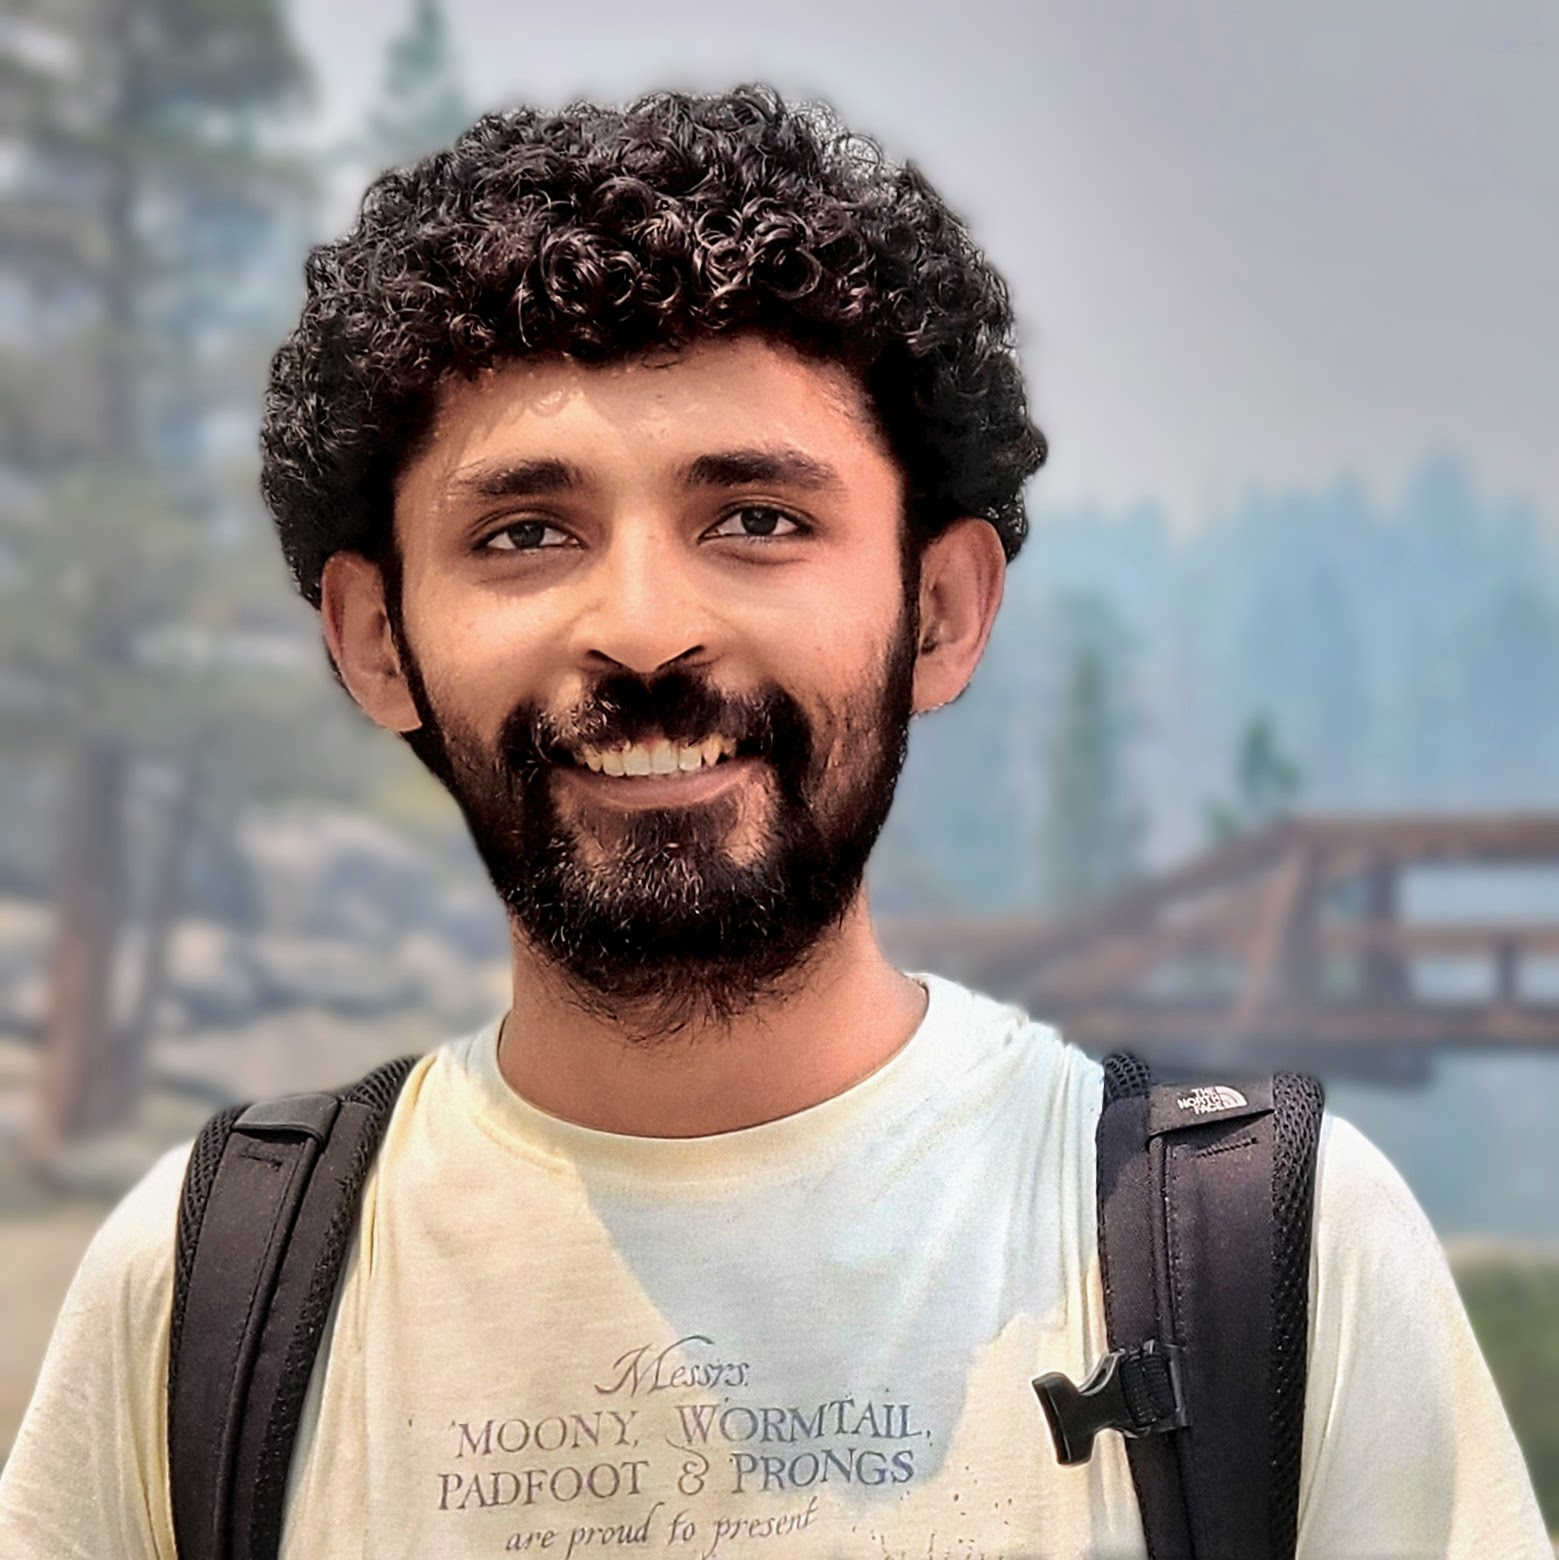
\includegraphics[width=0.25\linewidth]{general_figures/maharshi}
	\end{center}
\end{frame}


%todo(jbg):  or irt and chimera

\begin{frame}{Item Response Theory}

\only<1>{\gfxa{sat_sheet}{.9}}
\only<2>{\gfxa{sat_sheet_prob}{.9}}


\only<3>{\gfxa{jeopardy_irt_0}{.7}}
\only<4>{\gfxa{jeopardy_irt_1}{.7}}
\only<5>{\gfxa{jeopardy_irt_2}{.7}}

\end{frame}


  \begin{frame}{Making Dimensions Interpretable}
    % TODO(jbg): Add equations
        \begin{itemize}
        \item Examine thousands of questions (written for humans)
        \item Discover subsets of the data where there's a divergence
          between human and computer accuracy
        \item We then label each of those components
    \end{itemize}
	\gfxq{caimira_component}{.5}
 \end{frame}

  \begin{frame}{Hard for Computers: Abductive Inference}

    \begin{columns}
      \column{.5\linewidth}
      \gfxa{caimira_abductive_features}{1.0}
      \column{.5\linewidth}      
      \only<2>{\gfxa{caimira_abductive_skills}{1.0}}
    \end{columns}

  \end{frame}


  
  \begin{frame}{Hard for Humans: Science}

    \begin{columns}
      \column{.5\linewidth}
      \gfxa{caimira_science_features}{1.0}
      \column{.5\linewidth}      
      \only<2>{\gfxa{caimira_science_skills}{1.0}}
    \end{columns}

  \end{frame}

\begin{frame}{AdvScore}
	\begin{columns}
		\column{.3\linewidth}
		
		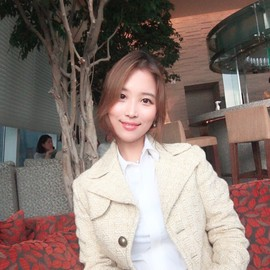
\includegraphics[width=1.0\linewidth]{general_figures/yooyeon}
		\column{.7\linewidth}
		\gfxa{advscore_paper}{1.0}
	\end{columns}
\centering
	NAACL 2025 Outstanding Paper
\end{frame}


  \begin{frame}{Adversarial Datasets}

    \begin{columns}
      \column{.5\linewidth}
      \gfxq{benchmark_saturation}{0.75}
Biggio et al., 2012: Poisoning attacks against Support Vector Machines

              \gfxa{adversarial_turtle}{.6}


            \column{.5\linewidth}
            \begin{itemize}
              
            \item Many benchmarks are ``saturated''
            \item Newer datasets claim to be ``adversarial''
              \begin{itemize}
              \item Hard for computers, ``easy'' for humans
              \item No real metric / definition
              \end{itemize}
            \item Can we use the lessons of the previous paper to inform how to write hard examples
            \item Can we \emph{measure} how well we did?
              \pause
            \item Language game: increasing the difficulty level
              \item But need to measure!
    \end{itemize}
            \end{columns}
 \end{frame}
    
    \begin{frame}{Adversarial Score}
	\begin{block}{Adversarial Score}
		
		\begin{equation}
			\text{\advscore{}}_\text{j} = \frac{\alert<2>{\mu_j}}{1 + \alert<4>{\delta_j}}
		\end{equation}
		
	\end{block}

      \begin{itemize}
        \item \alert<2>{Probability of skilled humans getting question right
          should be high, probability of skilled computers should be low}
\begin{equation}\label{eq:margin}
    \mu_j = \explain{Skilled human rep. prob.}{\twoplprob{\beta^{H_{(0)}}_{*}}{\theta_j}{\gamma_j}} - \explain{Skilled model rep. prob.}{\twoplprob{\beta^{M_{(0)}}_{*}}{\theta_j}{\gamma_j}},
\end{equation}
\only<3>{
  \vspace{-3cm}
  \begin{block}{Why not use raw accuracy?}
    \begin{itemize}
    \item Want patterns, not luck
    \item \abr{irt} can find (and downweight) bad questions
    \item What's the capital of Georgia?
    \end{itemize}
  \end{block}

}
\only<4->{
\item \alert<4>{Skilled humans shouldn't disagree on the answer}
  \begin{equation}\label{eq:delta}
    \delta_j = \sum_{i \sim H_{(1)}}
      \sfrac{\left[ \twoplprob{\beta_i^{H_{(1)}}}{\theta_j}{\gamma_j} -
        \overline{p_{H_{(1)}}}(r_{i,j}) \right] }{|H_{(1)}|}
\end{equation}
}

\end{itemize}
      
    \end{frame}

    \begin{frame}{AdvQA: Is this a viable incentive structure?}
      \begin{itemize}
    \item Can human authors interpret incentive?
      \begin{itemize}
      \item Computers should get questions wrong, smart humans should get them right
      \item Answers should be unique and easily verifiable
      \item Reward knowledge and skill
        \item Avoid ambiguity
      \end{itemize}
    \item Posthoc (no realtime feedback): Prizes given based on metric
      \item Professional trivia writers
      \end{itemize}
   \end{frame}
   
   
   \begin{frame}{What makes for Adversarial Example}
   	\only<1>{\gfxa{irtplot_0}{.9}}	
   	\only<2>{\gfxa{irtplot_1}{.9}}
   	\only<3>{\gfxa{irtplot_2}{.9}}
   	\only<4>{\gfxa{irtplot_3}{.9}}
   	\only<5>{\gfxa{irtplot_4}{.9}}
   	\only<6>{\gfxa{irtplot_5}{.9}}
   	\only<7>{\gfxa{irtplot_6}{.9}}
   \end{frame}

\begin{frame}{Adversarial Strategies}
	\begin{columns}
		\column{.5\linewidth}
			\only<1-2>{\gfxa{chrisrock}{.9}}
			\only<3-4>{\gfxa{parasite}{.9}}
			\only<5-6>{\gfxa{lulu_lemon}{.9}}
			\only<7-9>{\gfxa{akutagawa}{.9}}
		\column{.5\linewidth}
			\only<1-2>{What is the name of the American actor who stood up for his wife with a "slap that was heard around the world" during a popular awards show?}
			\only<2>{\\ \textbf{Brad Pitt / Will Smith}}
			\only<3-4>{What post-apocalyptic film directed by a Korean but not the director of Parasite is an allegory set on a train featuring the machinations of a rich businessman against the occupants of other cars?}
			\only<4>{\\ \textbf{Snowpiercer / Train to Busan}		}
			\only<5-6>{It's not headquartered in Biel, Switzerland but this activewear company has a logo that resembles the last letter of the Greek alphabet.}
			\only<6>{\\ \textbf{Omega / Lululemon}}
			\only<7-9>{A character in one story by \alert<8>{this author opens Crime and Punishment} to discover that it has turned into The Brothers Karamazov}
			\only<9>{\\ \textbf{Dostoyevski / Akutagawa}}
	\end{columns}
\end{frame}

    
    % TODO(jbg): AdvCal Picture slide

    \begin{frame}{Which Datasets are Adversarial?}
      \gfxa{cumulative_advscore}{.9}

      \begin{itemize}
      \item Not all datasets remain adversarial forever
      \item What helps make datasets adversarial?
        \begin{itemize}
          \item Bamboogle: Automatically generated          
          \item TrickMe: Human in the loop interface (expert), \abr{ir} models
        \item FM2: Human in the loop interface (crowdworker), \abr{ir} models
        \item AdvQA: Huaman in the loop (expert), \abr{llm} model + category instructions
        \end{itemize}

      \end{itemize}
    \end{frame}

\fsi{general_figures/blackbox}{AI is omnipresent but opaque}   
\fsi{simtrans/centaur-chess}{Centaur Chess}
\fsi{general_figures/kill_all_humans}{Fear of replacement (or worse)}
%\fsi{general_figures/bennet_robot}{}

\fsi{advcal/qanta_2025}{}


\frame{
	
	\frametitle{Thanks}
	
	%TODO(jbg): Check 
	\begin{block}{Collaborators}
		Hal Daum\'e III (UMD), Jon May (USC), Cristian (Columbia), Marine Carpuat
		(UMD), Eve Fleisig (Berkeley), Sherry Wu (CMU)
	\end{block}
	
	\begin{columns}
		
		\column{.75\linewidth}
		\begin{block}{Funders}
			\begin{center}
				
\includegraphics[width=0.2\linewidth]{general_figures/nsf}
				
\includegraphics[width=0.2\linewidth]{general_figures/darpa}
				
\includegraphics[width=0.2\linewidth]{general_figures/arl}
				
\includegraphics[width=0.2\linewidth]{general_figures/iarpa}
			\end{center}
		\end{block}
		
		\column{.3\linewidth}
		\begin{block}{Supporters}
			
\includegraphics[width=1.0\linewidth]{general_figures/iac}
			\gfxq{naqt}{1.0}
		\end{block}
		
	\end{columns}
}



\end{document}
